\section{Auswertung}
\label{sec:Auswertung}
Zunächst werden die Messwerte der Auslenkung $D$ gegen die Ablenkspannung $U_d$ aufgetragen und mithilfe einer linearen 
Ausgleichsrechnung approximiert.
 \begin{figure}[]
     \centering
     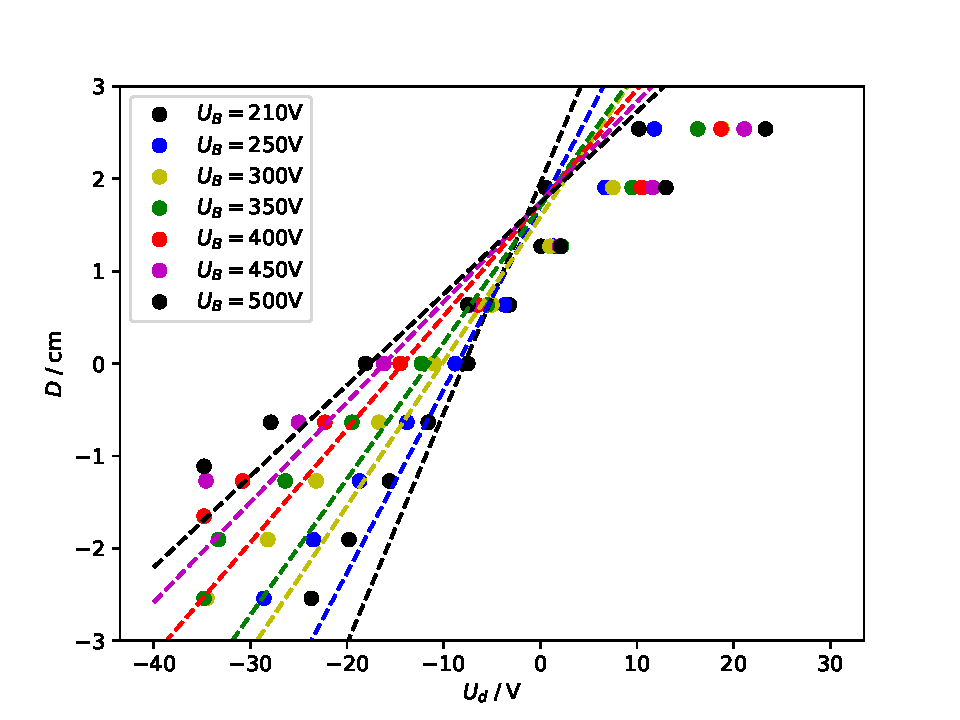
\includegraphics[width = 0.7\textwidth]{plots/all.pdf}
     \caption{Die Messwerte der Auslenkung D werden gegen die Abklenkspannung $U_d$ aufgetragen.
              Mit einer linearen Ausgleichsrechnung wird der Verlauf der Werte approximiert.}
     \label{fig:plot1}
 \end{figure}
Mit dem linearen Ausgleich ergibt sich nach,
\begin{align}
    D(U_d) = m\cdot U_d + b  \nonumber, \\
\end{align}

die Empfindlichkeit E der Braunschen Röhre mit,
\begin{equation}
    E(U_d)=\frac{D}{U_d}=m.
\end{equation}

\begin{table}
    \centering
    \begin{tabular}{c | c c c c c c c}
        \toprule
        $U_B\;/\;V$&210&250&300&350&400&450&500\\
        \midrule
        Empfindlichkeit $E\;/\;\frac{cm}{V}$& 0.2491& 0.1473& 0.1563& 0.1473& 0.1225& 0.1083& 0.0985\\
        \bottomrule
    \end{tabular}
    \caption{Dargestellt sind die verschiedenen Steigungen $m$/Empfindlichkeiten $E$ der verschiedenen 
    Ausgleichsgerade aus Abb. \ref{fig:plot1}}
    \label{tab:tab1}
\end{table}
\newpage
Für die Bestimmung der Apperaturkonstanten $K$, wird zunächst der Kehrwert der Beschleunigungsspannung $U_B$
gegen die Empfindlichkeit $E$ aufgetragen. Mithilfe einer Linearen Asugleichsgeraden der Form,
\begin{equation}
    E(1/U_b) = a\cdot \frac{1}{U_b} + b  \nonumber
\end{equation}
\begin{figure}[H]
    \centering
    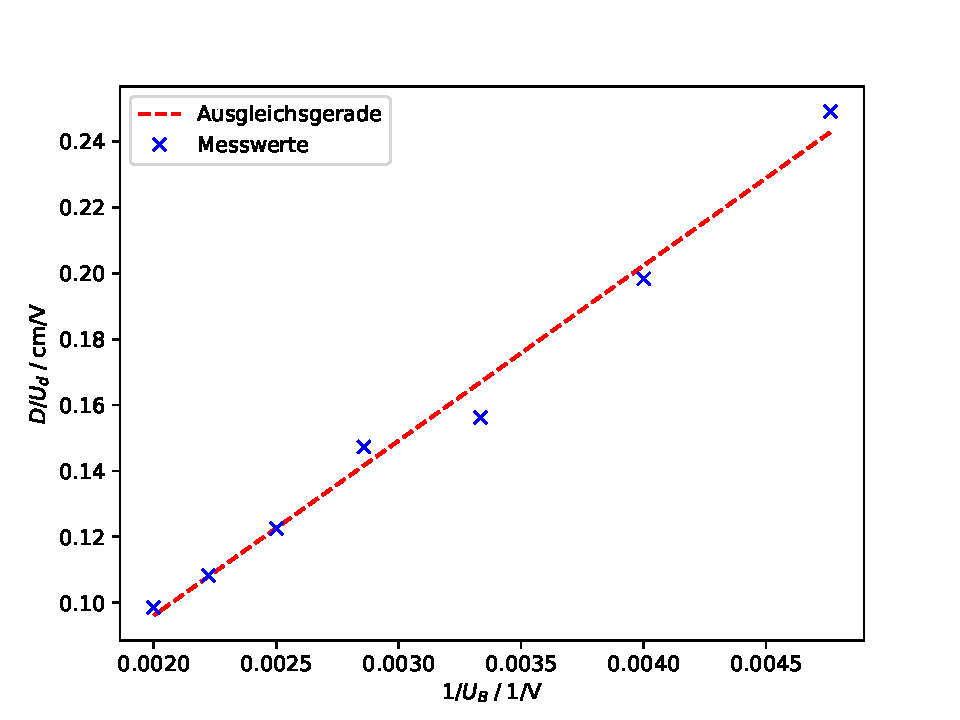
\includegraphics[width=0.8\textwidth]{plots/all2.pdf}
    \caption{Aufgetragen ist die Empfindlichkeit $E=D/U_d$ gegen den Kehrwert
    der Beschleunigungsspannung $U_B$.}
\end{figure}
mit den Parametern,
\begin{align}
    a&=(53.13\pm2.62),\\
    b&=(-0.01\pm0.0085).
    \label{eqn:y}
\end{align}
Es zeigt sich, dass der y-Achsenabschnitt hinreichend klein ist, sodass er für folgende Rechnung vernachlässigt wird.\\

Somit folgt aus der Beziehung
\begin{align}
    D&=\frac{p}{2d}L\frac{U_d}{U_B}\\
    \label{eqn:f1}
    \frac{D}{U_d}&=\frac{Lp}{2d} \cdot \frac{1}{U_B}=a\cdot \frac{1}{U_B}
\end{align}
Dem Apperaturaufbau entnimmt man die Parameter,
\begin{align}
    p = 1.9\text{cm}, \\
    d = 0.38\text{cm},\\
    L = 14.3\text{cm},\\
\end{align}
und somit folgt,
\begin{align}
    \frac{pL}{2d} &=35.75\text{cm}, \\
    a &= (53.13\pm2.62)\text{cm},\\
    \textrm{abs. Abweichung} &=(17.4\pm2.6)\text{cm} ,\\
    \textrm{rel. Abweichung} &= 48.61\%.
\end{align}

\subsection{Sinusspannung}
\begin{table}
    \centering
    \begin{tabular}{c c c c c}
        \toprule
        $\nu_{\text{sä},1/2}/$Hz & $\nu_{\text{sä},1}/$Hz & $\nu_{\text{sä},2}/$Hz & $\nu_{\text{sä},3}/$Hz\\
        \midrule
        150 & 62.5 & 50.0 & 25\\ 
        \bottomrule
    \end{tabular}
    \caption{Messung der Frequenzen der Sägezahnspannung}
\end{table}

Mit Gl. \ref{eqn:freq} ergibt sich,
\begin{table}
    \centering
    \begin{tabular}{c c c c c}
        \toprule
        $\nu_{\text{sä},1/2}/$Hz & $\nu_{\text{sä},1}/$Hz & $\nu_{\text{sä},2}/$Hz & $\nu_{\text{sä},3}/$Hz \\
        \midrule
        75.0 & 62.5 & 100.0 & 75.0\\ 
        \bottomrule
    \end{tabular}
    \caption{Messung der Frequenzen der Sägezahnspannung}
\end{table}

Gemittelt nach
\begin{equation*}
    \Delta \bar{\nu}_{\text{sin}}=\sqrt{\frac{1}{n(n-1)}\sum{\left(\nu_{\text{sin,i}}-\bar{\nu}_{\text{sin}}\right)^2}},
\end{equation*}
folgt damit
\begin{equation}
    \bar{\nu}_{\text{sin}}=(78.13\pm 7.86)\text{Hz},
    \label{eqn:sin} 
\end{equation}

Die Höhe zwischen einem Tief- und einem Hochpunkt der Sinnusspannung beträgt $0.127$cm,
es folgt also für den Scheitelwert $x=0.0635$cm.

Der Fehler folgt schließlich mit Gl. \ref{eqn:f1}
\begin{equation*}
    x \pm  \Delta x = c \pm \Delta c \cdot \frac{U_d}{U_B}
\end{equation*}
Somit folgt für die Empfindlichkeit der Röhre der Scheitelwert
\begin{equation}
    x \pm \Delta x=(0.0635\pm 0.0042)cm
\end{equation}
